\documentclass{beamer}

\usepackage[english]{babel}
\usepackage[T1]{fontenc}
\usepackage{beamerthemeAntibes}
\usepackage{graphicx}
\usepackage{listings}
\usepackage[utf8]{inputenc} 
\usepackage{epsfig}  
\usepackage{amsmath} 
\usepackage{multicol}
\usepackage{amsfonts}
\usepackage{hyperref}
\usepackage{listings}
\usepackage{changepage}

\lstset{
  basicstyle=\footnotesize,
  language=C,                % choose the language of the code                 % where to put the line-numbers
  backgroundcolor=\color{white},  % choose the background color. You must add \usepackage{color}
  showspaces=false,               % show spaces adding particular underscores
  showstringspaces=false,         % underline spaces within strings
  showtabs=false,                 % show tabs within strings adding particular underscores
  tabsize=2,                      % sets default tabsize to 2 spaces
  captionpos=b,                   % sets the caption-position to bottom
  breaklines=true,                % sets automatic line breaking
  breakatwhitespace=true,         % sets if automatic breaks should only happen at whitespace
  title=\lstname,                 % show the filename of files included with \lstinputlisting;
}



\setbeamertemplate{itemize/enumerate body begin}{\footnotesize}

\title{Social Networks}
\author{Luigi Giugliano$^1$, Steven Rosario Sirchia$^1$}
\institute{$^1$Università degli studi di Salerno}


\begin{document}

\begin{frame}
   \maketitle
\end{frame}

\begin{frame}
\frametitle{Introduction}
The purpose of our work is to test different algorithms in the three fundamental areas for assembling any search engine offering a Sponsored Search system:
\begin{itemize}
\item \textbf{Ranking} of web documents
\item \textbf{Matching} of words inside documents
\item \textbf{Auctions} for acquiring advertisement slots.
\end{itemize}
We will briefly talk about the proposed algorithms, and then compare running times and results obtained from their execution more in detail, suggesting what combination of algorithms seems to be the best for realizing a new search engine.
\end{frame}

\begin{frame}
\frametitle{Creating the Dataset}
Our experiments ran on a set of approximatively 30000 pages created this way:
\begin{itemize}
	\item we choose a web-page for each of the 15 categories listed in https://www.dmoz.org/
	\item for every of these web pages we crawled 2000 pages by using the Wibbi online crawler
	\item Moreover, from each pair of sets of 2000 pages, we choose at random 10 pairs of vertices (u, v) with u being a page in the first set and v being a page in the second set and added a link from u to v (if this link was absent)
\end{itemize}
\end{frame}

\begin{frame}
\frametitle{Creating the Dataset}
Here is the complete list of the websites chosen.
% Please add the following required packages to your document preamble:
% \usepackage{graphicx}
\begin{table}[]
	\centering
	\resizebox{\textwidth}{!}{%
		\begin{tabular}{lll}
			\textbf{Category} & \textbf{Website}       & \textbf{Description}                                                                                                                                                                                         \\
			Arts              & www.imdb.com           & The Internet Movie Database \\
			Business          & www.moodys.com         & Corporate finance, banking                                                                                                                        \\
			Computers         & www.ibm.com            &International Business Machines Corporation.                                                                                                                                                     \\
			Games             & www.ign.com            & Videogame news     \\
			Health            & www.who.int            & World Health Organization \\
			Home              & www.cooks.com          & Recipe search  \\
			Kids              & www.cartoonnetwork.com & The home of cartoons online
		\end{tabular}%
	}
\end{table}
\end{frame}

\begin{frame}
\frametitle{Creating the Dataset}
% Please add the following required packages to your document preamble:
% \usepackage{graphicx}
\begin{table}[]
	\centering
	\resizebox{\textwidth}{!}{%
		\begin{tabular}{lll}
			\textbf{Category} & \textbf{Website}       & \textbf{Description}                                                                                                                                                                                       \\
			News              & www.foxnews.com        & Breaking News\\
			Recreation        & www.lego.com           & Producer of bilding blocks.                                                                                                                                                                             \\
			Reference         & www.britannica.com     & Encyclopaedia Britannica Online.\\
			Science           & www.nasa.gov           & Comprehensive, world-class center for aeronautics                   \\
			Shopping          & www.amazon.com         & Most known shopping website\\
			Society           & www.un.org             & Daily United Nations news, documents and publications \\
			Sports            & www.nba.com            & The official site of the National Basketball Association\\
			Regional          & www.lonelyplanet.com   & Offers travel advice, detailed maps, travel news                                                   
		\end{tabular}%
	}
\end{table}
\end{frame}

\begin{frame}
 \frametitle{Overview}
 \footnotesize \tableofcontents[
   						sectionstyle=show,
   						subsectionstyle=show/show,
   						subsubsectionstyle=hide
        					]
 \end{frame}

\AtBeginSection[]
  {
     \begin{frame}<beamer>
     \frametitle{Overview}
   \footnotesize \tableofcontents[
   						sectionstyle=show/shaded,
   						subsectionstyle=show/show/hide,
   						subsubsectionstyle=show/show/show/hide
        					]
     \end{frame}
}

\section{Ranking}
\subsection{Page Rank}
\begin{frame}
\frametitle{Page Rank}
\begin{block}{Page Rank}
The intuition behind \emph{Page Rank} is:
\center``a page is important if it is cited by other important pages''.
\end{block}
This intuition rises from the usual endorsement mode, for example, among academic or governmental pages, among bloggers, or among personal pages more generally. It is also the dominant mode in the scientific literature.
\end{frame}

\begin{frame}
\frametitle{Algorithm}
We can think of PageRank as a kind of “fluid” that circulates through the network, passing from node to node across edges, and pooling at most important nodes.
\center
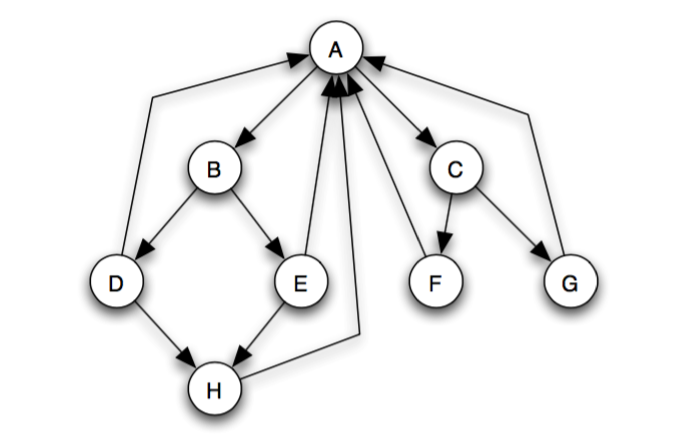
\includegraphics[scale=0.3]{img/general_network.png} 
\end{frame}


\begin{frame}
\frametitle{Algorithm Steps}
\begin{itemize}
\item \onslide<1-> In a network with n nodes, we assign all nodes the same initial PageRank, set to be 1/n.
\item \onslide<2-> We choose a number of steps k.
\item \onslide<3-> We then perform a sequence of k updates to the PageRank values, using the following
rule for each update:\\
\begin{adjustwidth}{2.5em}{0pt}
\textbf{Basic PageRank Update Rule}: Each page divides its current PageRank equally across its out-going links, and passes these equal shares to the pages it points to. (If a page has no out-going links, it passes all its current PageRank to itself.) Each page updates its new PageRank to be the sum of the shares it receives.
\end{adjustwidth}
\end{itemize}
\end{frame}

\begin{frame}
\frametitle{The ``Wrong'' nodes}
There is a difficulty with the basic definition of PageRank, however: in many networks, the “wrong” nodes can end up with all the PageRank.
\begin{center} 
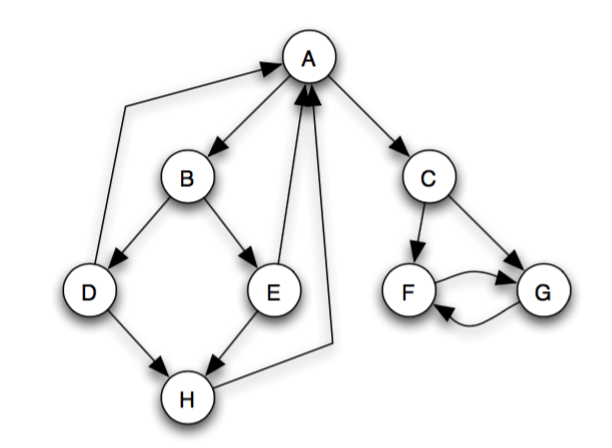
\includegraphics[scale=0.2]{img/wrong_nodes.png} 
\end{center}
The Wrong nodes are a small sets of nodes that can be reached from the rest of the graph, but have no paths back.
\end{frame}

\begin{frame}
\frametitle{Scaled PageRank }
We can use the mechanism of fluid presented before: there is a \alert{counter-balancing process} preventing that all the water stands only on downhill places on the earth.
\begin{block}{Scaled PageRank Update Rule}
First apply the Basic PageRank Update Rule.\\ 
\smallskip
Then scale down all PageRank values by a factor of s, shrinking the total from 1 to s. \\
\smallskip
We divide the residual $1 - s$ units of PageRank equally over all nodes, giving$ (1 - s)$/$n$ to each.
\end{block}
\end{frame}

\subsubsection{Results}
\begin{frame}
\frametitle{Results}
We are going to present the result of the experiment, comparing the \alert{execution time} of PageRank on following inputs:
\begin{itemize}
\item Graph of 1000 nodes
\item Graph of 2000 nodes
\item Graph of 5000 nodes
\item Graph of 10000 nodes
\item Graph of 20000 nodes
\item Full Graph (30000 nodes) 
\end{itemize}
All the graphs are generated by chunking the Full Graph.
\end{frame}

\begin{frame}
\frametitle{Graph of Times}
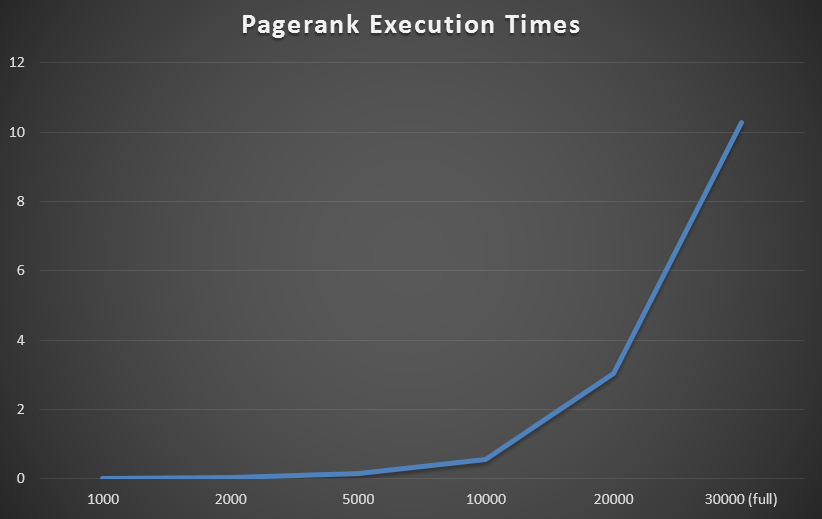
\includegraphics[scale=0.5]{img/Ranking/Pagerank.PNG} 
\end{frame}

\begin{frame}
\frametitle{Rank Values}
We now present the result of the PageRank algorithm, considering the score of the pages:\\
\begin{itemize}
\item \textbf{Min}: $5e-06$
\item \textbf{Max}: $1.8e-03$
\item \textbf{Mean}: $1.1e-05$
\item \textbf{Std}: $5.4e-05$
\end{itemize}
\end{frame}

\subsection{HITS}
\begin{frame}
\frametitle{HITS}
This hubs-and-authorities algorithm, sometimes called HITS (\textit{hyperlink induced
topic search}), was originally intended not as a preprocessing step before
handling search queries, as PageRank is, but as a step to be done along with
the processing of a search query, to rank only the responses to that query.\\
\medskip
This kind of approach is  used by the Ask search engine.
\end{frame}

\begin{frame}
\frametitle{The Intuition Behind HITS}
HITS views important pages as having two different types of importance.
\begin{itemize}
\item Certain pages are valuable because they provide information about a
topic. These pages are called \textbf{authorities}.
\item Other pages are valuable not because they provide information about any
topic, but because they tell you where to go to find out about that topic.
These pages are called \textbf{hubs}.
\end{itemize}
\end{frame}

\begin{frame}
\frametitle{HITS Algorithm}
For calculating the HITS values for the pages, we shall assign two scores to each Web page.
One score represents the \textit{hubbiness} of a page, that is the degree to which it
is a good hub, and the second score represents the degree to which the page
is a good authority.\\
\medskip
These values  are then calculated as:
\begin{itemize}
\item \onslide<1-> \textbf{Hubbiness}: the sum of the Authority value of the outgoing nodes.
\item \onslide<2-> \textbf{Authority}: the sum of Hubbiness value of the incoming nodes.
\end{itemize}
\-\\\
\smallskip
\onslide<3-> These values are normalized so that the largest value is 1.
\end{frame}

\subsubsection{Results}
\begin{frame}
\frametitle{Results}
We are going to present the result of the experiment, comparing the \alert{execution time} of HITS on following inputs:
\begin{itemize}
\item Graph of 1000 nodes
\item Graph of 2000 nodes
\item Graph of 5000 nodes
\item Graph of 10000 nodes
\item Graph of 20000 nodes
\item Full Graph (30000 nodes) 
\end{itemize}
All the graphs are generated by chunking the Full Graph.
\end{frame}

\begin{frame}
\frametitle{Tuning for improving performance}
On the first attempts of running the algorithm on the full graph we observed that one iteration took about 30 minutes, due to the nature of the algorithm. \\
In each iteration we explore all the graph and calculate the incoming nodes for the current node \dots\\
\bigskip
Considering that the graph never changes, we precomputed all the incoming nodes for each node so we can obtain the incoming nodes in $O(1)$.
\end{frame}

\begin{frame}
\frametitle{Tuning for improving performance}
In the HITS algorithm there are two stop rules:
\begin{itemize}
\item Max number of iteration
\item Min confidence on the errors reached
\end{itemize}
\medskip
We noticed that in some cases the Algorithm runs until the maximum number of steps is reached, and when this happens the relative error trends to stabilize on a fixed level. We decided then to add a new stop rule: \\
\begin{itemize}
\item If two successive relative errors are distant at maximum a small $\epsilon$, then stop the algorithm.
\end{itemize}
We tried this improvement on the full graph, we plotted the time as a pink line \dots the difference is embarrassing 
\end{frame}

\begin{frame}
\frametitle{Graph of Times}
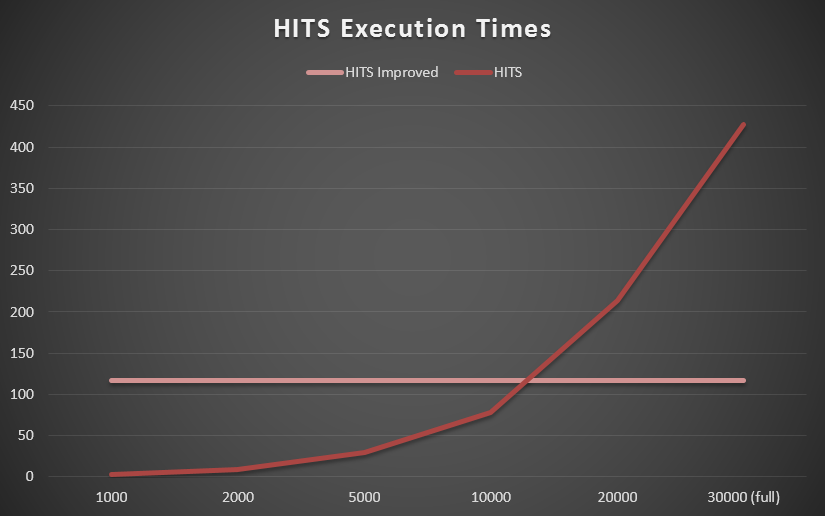
\includegraphics[scale=0.5]{img/Ranking/HITS.PNG} 
\end{frame}

\begin{frame}
\frametitle{Parallel Version}
We also implemented the parallel version, but the performance resulted to be worst compared with the non-parallel version: this is due to overhead of coping all the structures needed for the calculation of scores.\\
\medskip
We now present times of 10 iterations of both version:
\begin{itemize}
\item \textbf{Non-Parallel}: 4,15''
\item \textbf{Parallel}: 53,41''
\end{itemize} 
\end{frame}

\begin{frame}
\frametitle{Hits Authority Values}
We now present the result of the HITS algorithm, considering the authority score of the pages:\\
\begin{itemize}
\item \textbf{Min}: $0$
\item \textbf{Max}: $1$
\item \textbf{Mean}: $0.0017$
\item \textbf{Std}: $0.0408$
\end{itemize}
\end{frame}

\begin{frame}
\frametitle{Hits Hubbiness Values}
We now present the result of the HITS algorithm, considering the hubbiness score of the pages:\\
\begin{itemize}
\item \textbf{Min}: $0$
\item \textbf{Max}: $1$
\item \textbf{Mean}: $0.0585$
\item \textbf{Std}: $0.2328$
\end{itemize}
\end{frame}

\subsection{Comparing the Results}
\begin{frame}
\frametitle{Comparing the Results}
The results are incomparable, both considering execution time and values: \\
HITS time is up to $40$ time the PageRank time.\\
The values are different for the nature of the algorithms.\\
\medskip
But we can combine the observations we made earlier to infer the structure of the network, in fact both PageRank and HITS authority have the majority of documents with a low score, and also the variance prove this.\\
\medskip
For the HITS hubbiness we notice, instead, that the variance is higher, as well as the mean, this mean that the values are more widespread along the network.
\end{frame}

\begin{frame}
\frametitle{Network structure}
\begin{center}
\includegraphics[scale=0.4]{img/Network(1).png} 
\end{center}
\end{frame}

\begin{frame}
\frametitle{Network structure}
\begin{center}
\includegraphics[scale=0.32]{img/Network(2).png} 
\end{center}
\end{frame}

\section{Matching}
\subsection{Best Match}
\begin{frame}
\frametitle{The idea of Best Match}
Given a query $q$, containing $n$ query words, and a set of documents $S$, we define Best Match as a method that finds a subset of document $S'$ such that:
\begin{itemize}
	\item each document $s_i$ of $S'$ has a "reasonable" number of query words in it
\end{itemize}
\medskip
According to this definition the basic Best Match consists of:
\begin{itemize}
	\item counting how many query words documents have
	\begin{itemize}
		\item we call this value "score" of a document
		\item it is at maximum $n$
	\end{itemize}
	\item ordering in decreasing order of score the documents (optional)
	\item return all documents whose score is "reasonable"
	\begin{itemize}
		\item we use a threshold to define what is "reasonable"
	\end{itemize}
\end{itemize}
\end{frame}
\begin{frame}
\frametitle{Refining the Best Match}
Two are the basic refinements to have a more efficient Best Match:
\begin{enumerate}
	\item using an inverted index
	\begin{itemize}
		\item in the form (word -> list of documents containing the word)
		\item the keys of the dataset are the query words
		\item we can have in O(1) all the documents with a determined word  
	\end{itemize}
	\item using the frequency instead of assigning score 1 to each query word found
	\begin{itemize}
		\item defined as number of occurrences in document $d$ / length($d$)
		\item requires precalculation of occurrences for all words and all $S$
		\item it represents the \textbf{relevance} of documents to a particular word or query
	\end{itemize}	
\end{enumerate}
\end{frame}

\subsection{Improved Best Match}
\newcounter{sauvegardeenumi}
\newcommand{\asuivre}{\setcounter{sauvegardeenumi}{\theenumi}}
\newcommand{\suite}{\setcounter{enumi}{\thesauvegardeenumi}}

\begin{frame}
\frametitle{Improved Best Match}
We implemented also the following improved version of Best Match:
\begin{enumerate}
	\item Sort documents in each inverted index in order of frequency of the term at which the inverted index refers
	\item For every query term define its possible impact on the score as the frequency of the most frequent document in its index
	\item Sort the query terms in decreasing order of impact
	\item Consider the first 20 documents in the index of the first query term (if the first query term has an index with less than 20 documents, then complete with the first documents in the index of the next query term)
	\asuivre
\end{enumerate}
\end{frame}

\begin{frame}
\frametitle{Improved Best Match}
\begin{enumerate}	
	\suite
	\item Compute the score for each of these documents
	\item Consider the first term in which there are documents that have not been scored
	\item Consider the first non-scored document in the index of this term
	\item If the frequency of the current term in the current document plus the sum of the impact of next terms is larger than the score of the 20-th scored document, then score this document and repeat from 7, otherwise consider the next    
\end{enumerate}
\end{frame}

\subsection{Results}
\begin{frame}
\frametitle{Experiment configuration}
For obtaining the time comparison between BestMatch and ImprovedBestMatch we run both algorithms on 25 random queries of different length :\\
\begin{itemize}
\item 5 for each length from 3 to 7
\end{itemize} 
Then we mean the results and plotted them on a graph
\end{frame}

\begin{frame}
	\frametitle{Time comparison BestMatch vs ImprovedBestMatch}
	\begin{center}
	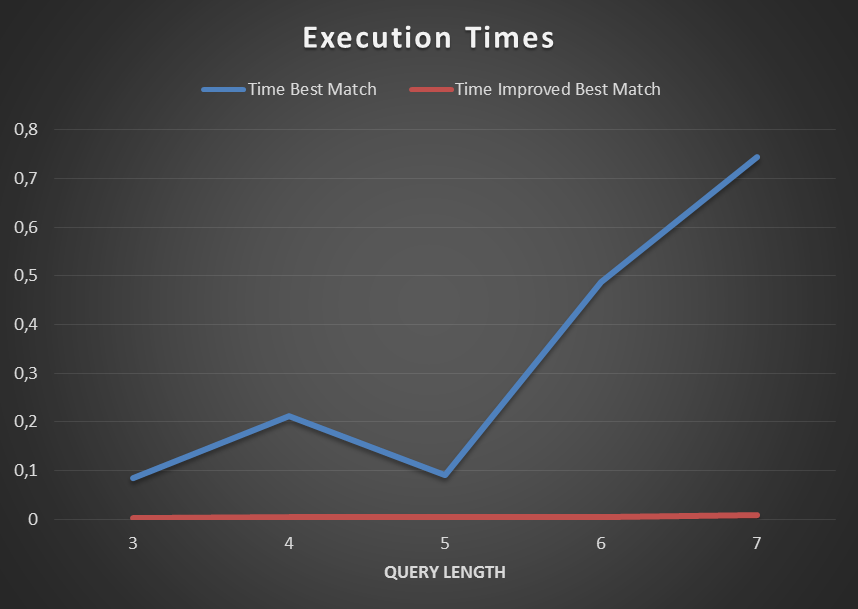
\includegraphics[scale=0.32]{img/Matching/Tempi.PNG} 
	\end{center}
\end{frame}

\begin{frame}
\frametitle{Time comparison BestMatch vs ImprovedBestMatch}
First of all  Improved Best Match ``\alert{wins}'' on all query lengths, moreover it seems to be constant. This is due to the fact that there is a huge difference on the times of the algorithm at least of 1 order of magnitude.\\
\medskip
We can notice that times of query of length 5 in best match are smaller of the one on length 4; this can be attributable to the random generation of queries, in fact, if we take 5 very uncommon words there are \alert{few} documents that have one of these word so the algorithm ends quickly. 
\end{frame}

\begin{frame}
\frametitle{Improved Best Match time}
\begin{center}
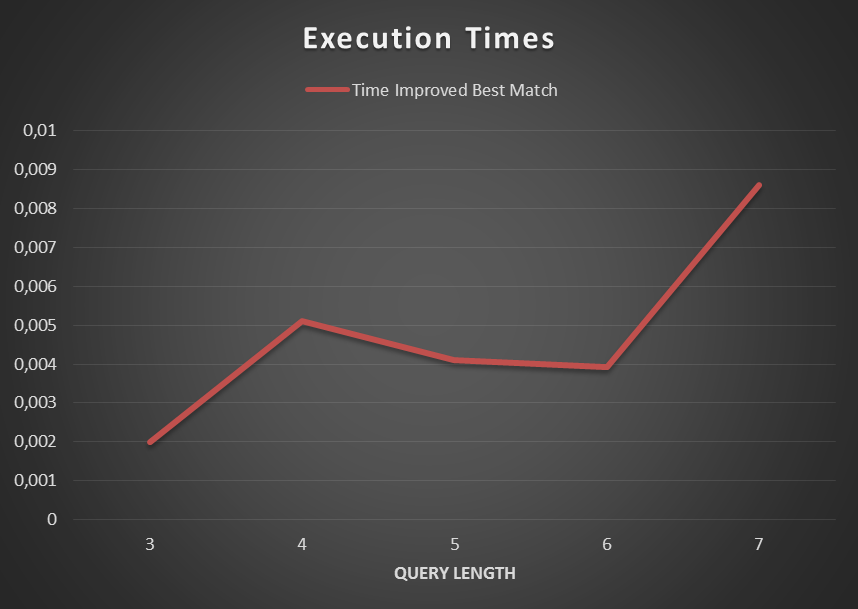
\includegraphics[scale=0.32]{img/Matching/Tempi_IMP.PNG} 
\end{center}
\end{frame}

\section{Search Engine}
\begin{frame}
\frametitle{Search Engine}
The implemented Search Engine combine the algorithms seen before.\\ 
Given a query:
\begin{enumerate}
\item Find the documents that match the query using:
\begin{itemize}
\item Best Match
\item Improved Best Match
\end{itemize}
\item Order these documents by:
\begin{itemize}
\item Page Rank Score
\item HITS authority
\end{itemize}
\end{enumerate}
\end{frame}

\subsection{Results}
\begin{frame}
\frametitle{Running configurations}
\begin{itemize}
\item We ran the experiment for a total of 25 queries
\item 5 for each length between 3 and 7
\begin{itemize}
\item In each group of 5 queries 1 of them is manually constructed by us for having a high likelihood with a real query
\item The other 4 are randomly generated among the dataset
\end{itemize} 
\item The manual generated  query are used not only for calculate the execution time, but also for fully analysing the output of search engine
\end{itemize}
\end{frame}

\begin{frame}
\frametitle{Ranking on Improved Best Match}
\begin{center}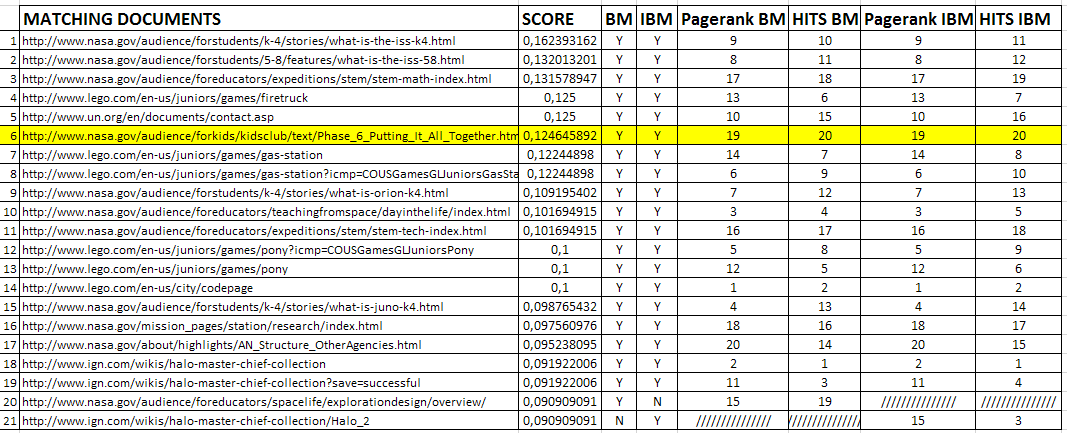
\includegraphics[scale=0.40]{img/Search/Query.PNG} \end{center}
\end{frame}

\begin{frame}
\frametitle{Ranking on Best Match}
\begin{center}
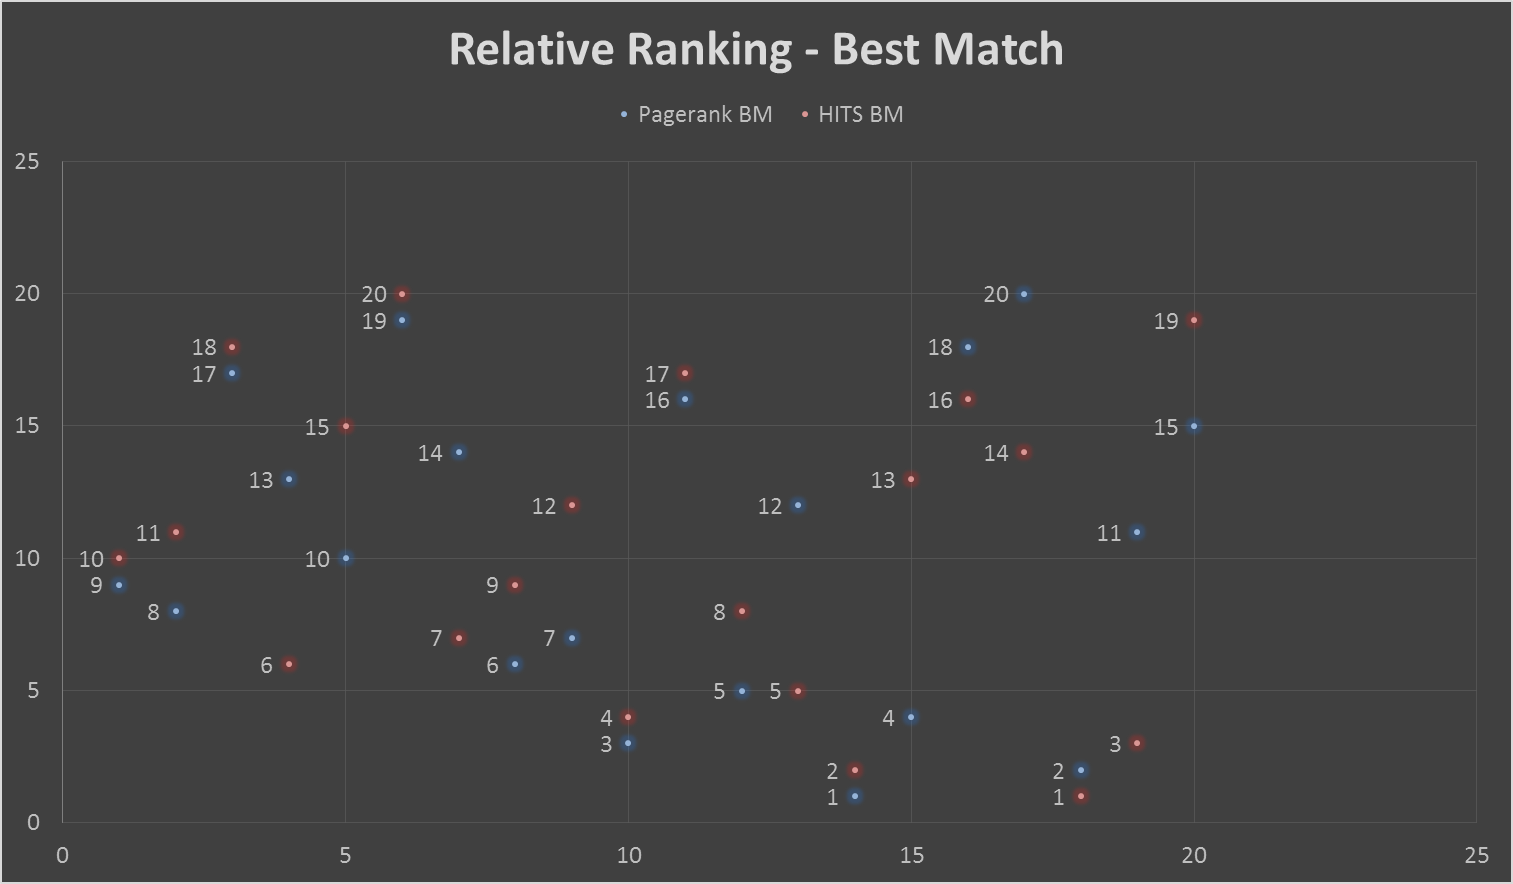
\includegraphics[scale=0.20]{img/Search/Best.PNG} 
\end{center}
\end{frame}

\begin{frame}
\frametitle{Ranking on Improved Best Match}
\begin{center}
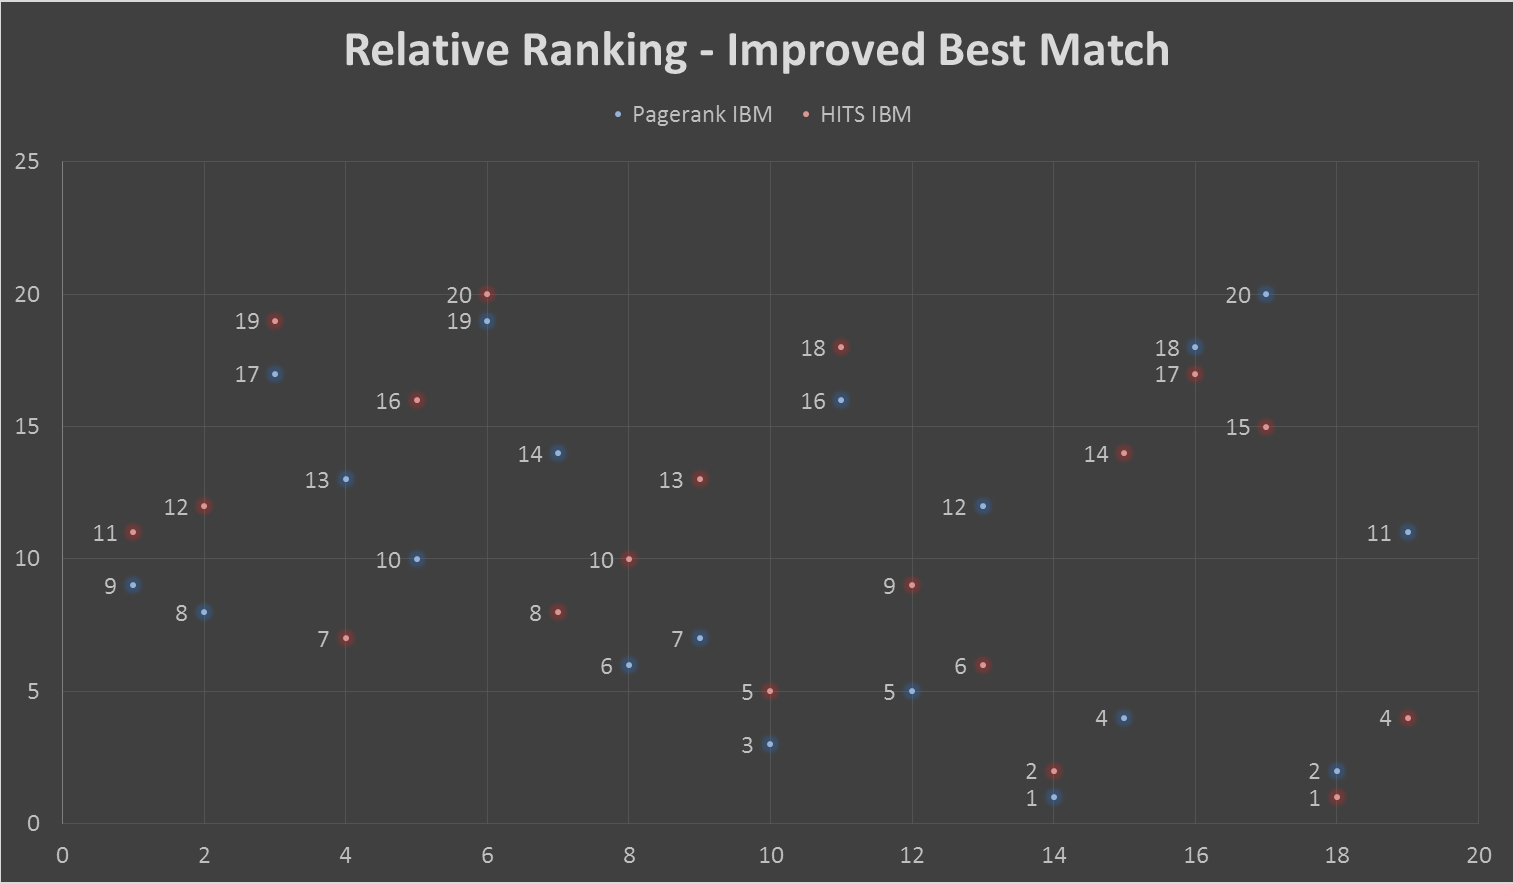
\includegraphics[scale=0.20]{img/Search/Improved.PNG} 
\end{center}
\end{frame}


\begin{frame}
\frametitle{Considerations}
First of all we can observe that in both types of matching we found the document we used for generating the query, as expected.\\
\medskip
Another thing we notice is that the two results differ only by one document, but these documents have the same matching score, so this difference is due to the order of visiting documents.\\
\medskip
We notice that there is an \alert{high} correlation within the first and the last position of the documents ordered by PageRank or by HITS, this means that even if the values of the ranking algorithms are not comparable absolutely, tent to have a \alert{relative} comparability.
\end{frame}




\section{Auction}

\subsection{First Price Auction}
\begin{frame}
\frametitle{First Price Auction}
In this kind of auction, bidders submit simultaneous ``sealed bids'' to the seller. The terminology comes from the original format for such auctions, in which bids were written down and provided in sealed envelopes to the seller, who would then open them all together.\\
\medskip
\begin{center}\textbf{The highest bidder wins the object \\ and pays the value of her bid.}\end{center}
\end{frame}

\begin{frame}
\frametitle{Non - truthfulness of FPA}
In a sealed-bid first-price auction, the value of your bid not only affects whether you win but also how much you pay.\\
\medskip
Bidding your true value is not a dominant strategy. By bidding your true value, you would get a payoff of 0 if you lose (as usual), and you would also get a payoff of 0 if you win, since you’d pay exactly what it was worth to you.\\
\medskip
As a result, the optimal way to bid in a first-price auction is to “shade” your bid slightly downward, so that if you win you will get a positive payoff. Determining how much to shade your bid involves balancing a trade-off between two opposing forces.
\end{frame}

\subsection{Generalized Second Price Auction}
\begin{frame}
\frametitle{Generalized Second Price Auction}
Bidders submit simultaneous sealed bids to the sellers;
\begin{center} 
\textbf{The highest bidder wins the object \\
and pays the value of the second-highest bid.} 
\end{center}
\end{frame}

\begin{frame}
\frametitle{Truthfulness of GSP}
Truthful bidding is a dominant strategy in a sealed-bid second-price auction. The heart of the argument is the fact noted at the outset: in a second-price auction, your bid determines whether you win or lose, but not how much you pay in the event that you win. \\
\medskip
So in a second-price auction, it makes sense to bid your true value even if other bidders are overbidding, underbidding, colluding, or behaving in other unpredictable ways.
\end{frame}

\subsection{Results}

\subsubsection{Bots}
\begin{frame}
\frametitle{Description of Bots}
We used the following bots:
\begin{itemize}
\item \textbf{Best\_response} with balanced tie-breaking rules
\item \textbf{Best\_response\_competitive} submit the highest possible bid that gives the preferred\_slot
\item \textbf{Best\_response\_altruistic } submit the lowest possible bid that gives the preferred\_slot
\item \textbf{Competitor} always submit a bit grater than the highest bid
\item \textbf{Budget\_saving} always submit the minimum between last-non winning bid and advertiser value
\end{itemize}
\end{frame}

\begin{frame}
\frametitle{Description of Bots}
We used the following bots:
\begin{itemize}
\item \textbf{Competitor\_budget} Use competitor when budget is more than its half, best\_response otherwise  
\item \textbf{Preferential\_competitor} Use competitor when value is more than a threshold, budget\_saving otherwise
\item \textbf{Best\_competitor\_budget} Use best\_response\_competitive when budget is more than its half, best\_response otherwise
\item \textbf{Best\_preferential\_competitor} Use best\_response\_competitive when value is more than a threshold, budget\_saving otherwise
\item \textbf{Random} bids randomly
\end{itemize}
\end{frame}


\subsubsection{Selecting Bots}
\begin{frame}
\frametitle{Selection of interesting Bots}
The configuration of the experiment for finding the most interesting bots is the following:
\begin{itemize}
\item \textbf{Number of Query Words} 1
\item \textbf{Number of Auction} 10
\item \textbf{Slot 1 click-through } 0.4
\item \textbf{Slot 2 click-through } 0.15
\item \textbf{Number of Advertiser} 3
\begin{itemize}
\item 1 bot to test and 2 enemies (of the same kind)
\end{itemize}
\item \textbf{Values} 7
\item \textbf{Budgets}  25
\item \textbf{Number of runs } 10000
\end{itemize}
\end{frame}

\begin{frame}
\frametitle{FPA Utility}
\begin{center}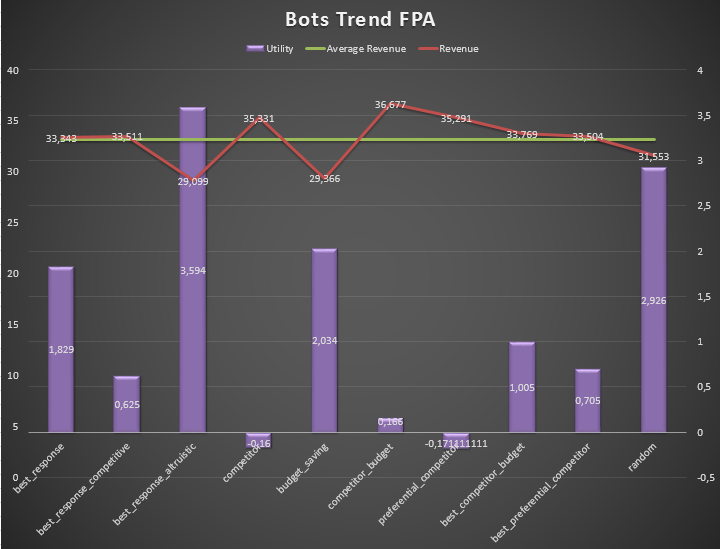
\includegraphics[scale=0.46]{img/Auctions/FPA_all_Utility.PNG} 
\end{center}
\end{frame}

\begin{frame}
\frametitle{Considerations on FPA advertiser-side }
Observing FPA graph it seems that \textit{best\_response\_altruistic} is the best bot, yielding the \alert{highest} utility.\\
\medskip
This is due to the fact the bots that try to save their budgets, offer the lowest bid possible.
Since these bids are ``far'' from the advertiser's values and FPA is not truthful, they have a high chance to have a good slot at low price. 
\end{frame}

\begin{frame}
\frametitle{Considerations on FPA seller-side}
The bots who try to save their budget on seller-side are the \alert{worst}, because they lower not only their own bids, but also the bids of the whole auction.\\
\medskip
It follows that the other kinds of bots which raise their bids are more \alert{lucrative} for us.\\
\medskip
For the reasons explained before we need a balance between high revenue and high utility, and the bot that seems to accomplish this is \textbf{best\_response}.
\end{frame}

\begin{frame}
\frametitle{GPS Utility}
\begin{center}
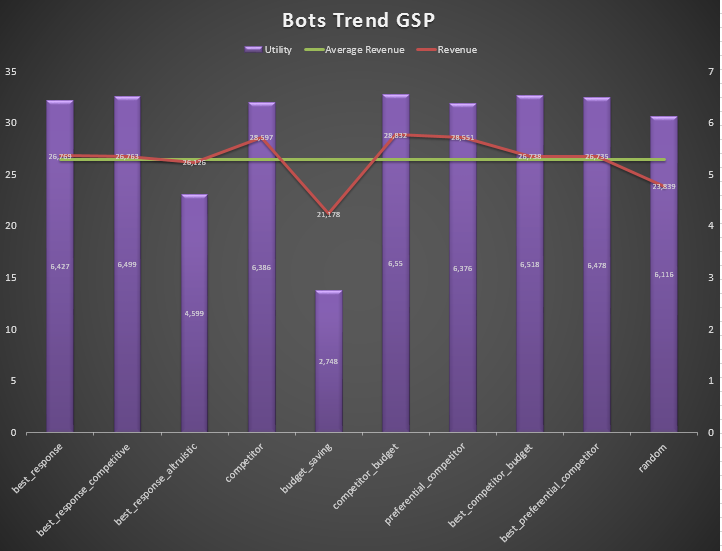
\includegraphics[scale=0.46]{img/Auctions/GSP_all_Utility.PNG} 
\end{center}
\end{frame}


\begin{frame}
\frametitle{Considerations on GSP advertiser-side}
We notice that, since GPS is truthful, the bots that offer bids near to their ``real'' value perform \alert{better}, obtaining a higher utility.\\
\medskip
For this reason all the bots that tent to lower the bids, straying from the ``real'' value, perform a lot \alert{worst}, obtaining a lower utility. 
\end{frame}


\begin{frame}
\frametitle{Considerations on GSP seller-side}
We notice that there are a lot of bots with  almost the same utility, around $\sim6,5$.\\
\medskip
Since we know the bots have different  behaviours, we would like to understand how this difference affect the outcome of the bots.\\
\bigskip
For this reason we decided to calculate an heuristic about the quantity and quality of slots obtained.
\end{frame}

\begin{frame}
\frametitle{Our heuristic}
The heuristic for a bidder is calculated as follow:\\
\medskip
On each step of an auction, given the \textbf{preferred\_slot} and the result of that step.
\begin{itemize}
\item Add $1$ if the bidder obtains the \textbf{preferred\_slot}, or he wants nothing and obtain nothing 
\item Add $2$ if the bidder obtains a better slot, since he bids for a worse slot.
\item Subtract $1$ if the bidder obtain a worse slot, since he bids for a better slot.
\end{itemize}
We mediate this score on the auction step.\\
The heuristic straddles in the range $ [-1;2]$
\end{frame}


\begin{frame}
\frametitle{Heuristic on FPA}
\begin{center}
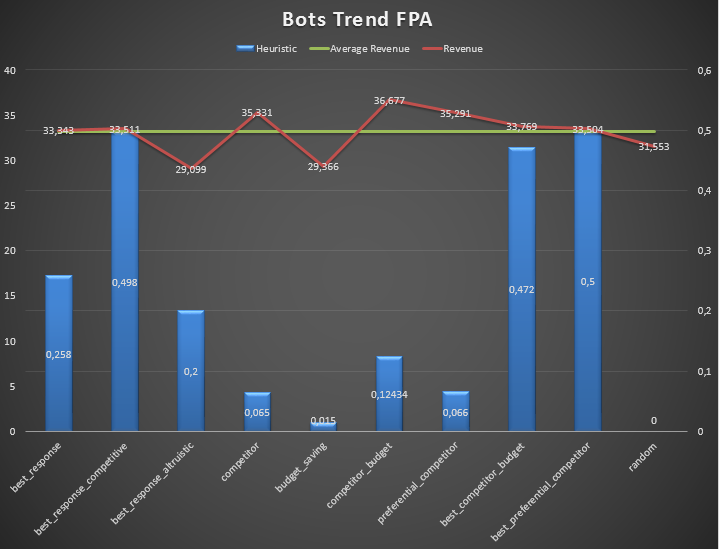
\includegraphics[scale=0.46]{img/Auctions/FPA_all_Heuristic.PNG} 
\end{center}
\end{frame}

\begin{frame}
\frametitle{Considerations on FPA heuristic}
Considering the bots who have the higher utility (best\_response\_altruistic, budget\_saving) we notice that they have a very \alert{low} heuristic score, this is due to the fact they tent the obtain the slots that they don't ``want'' but at a very \alert{low price} resulting in a high utility.\\
\medskip
On the other hand aggressive bidders, tent to have a better heuristic score but a worse utility, since they pay a lot for the slot they obtain.\\
\medskip
\textbf{For the FPA the revenue is not dependant on the heuristic score}, but on the ``nature'' of the bot.
\end{frame}


\begin{frame}
\frametitle{Heuristic on GSP}
\begin{center}
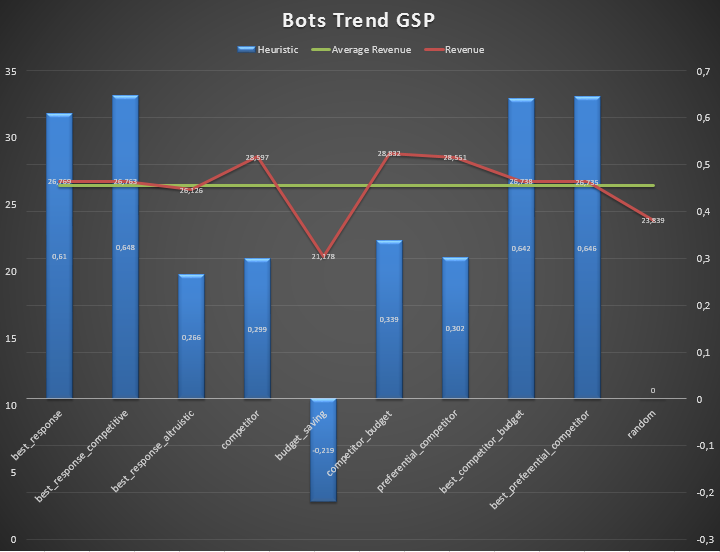
\includegraphics[scale=0.46]{img/Auctions/GSP_all_Heuristic.PNG} 
\end{center}
\end{frame}

\begin{frame}
\frametitle{Considerations on GSP heuristic}
Thanks to the heuristic score  we can divide the bots in several groups, the ``blind'' competitors, the ``wise'' competitors and  the ``stingy''.\\
\begin{table}[]
\centering
\begin{tabular}{l|l|l|l|}
\cline{2-4}
                                                  & \textbf{Utility} & \textbf{H\_score} & \textbf{Revenue} \\ \hline
\multicolumn{1}{|l|}{\textbf{"Blind" competitor}} & High             & Low               & High             \\ \hline
\multicolumn{1}{|l|}{\textbf{"Wise" competitor}}  & High             & High              & Average          \\ \hline
\multicolumn{1}{|l|}{\textbf{"Stingy"}}           & Low              & Low               & Low              \\ \hline
\end{tabular}
\caption{Resume}
\label{my-label}
\end{table}
\end{frame}


\begin{frame}
\frametitle{Comparing FPA and GPS results}
\begin{center}
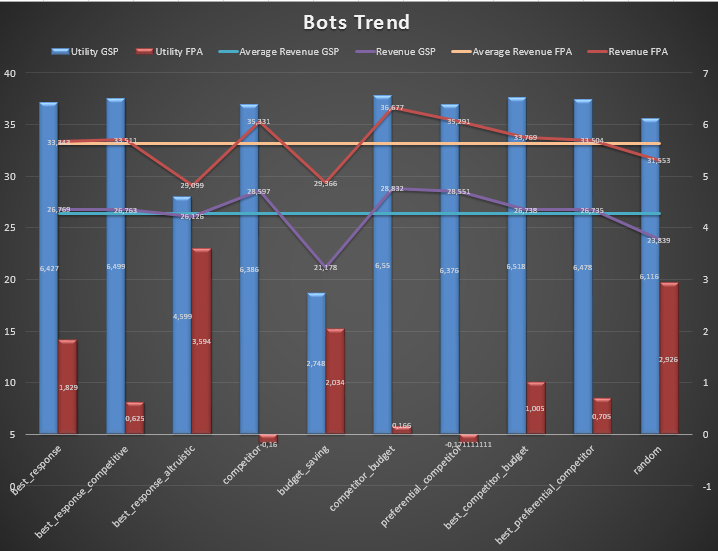
\includegraphics[scale=0.46]{img/Auctions/Combined_Utility.PNG} 
\end{center}
\end{frame}

\begin{frame}
\frametitle{Comparing FPA and GPS results}
\begin{center}
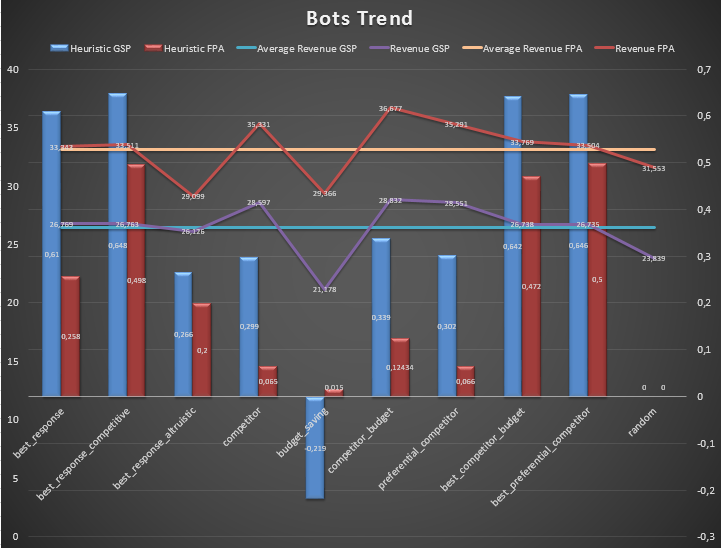
\includegraphics[scale=0.46]{img/Auctions/Combined_Heuristic.PNG} 
\end{center}
\end{frame}


\begin{frame}
\frametitle{Comparing FPA and GPS results}
Comparing the auction types, we notice that on a ``fixed'' auction they have the following behaviour:
\begin{itemize}
\item FPA auction produce the \alert{highest} revenue for the seller, this follows from the fact that you pay exactly what you bid. As for clients satisfaction, we notice that they have both a \alert{low} heuristic and  utility compared to GPS.
\item GPS instead produce \alert{lowest} revenue and \alert{high} utility and heuristic score for the client, this is due the nature of GPS:\\
the winner of a slot can offer a very high bid without having too much impact on what he pays, because he doesn't pay his bid but the bid immediately lower than his.
\end{itemize}
The choice depends of what we want  to ``favour''
\end{frame}

\begin{frame}
\frametitle{Revenue equivalence Theorem}
As we notice the revenue are different, this is due to the fact that we stopped the auction at 10 steps and moreover the budget of the advertisers are different so using balance algorithms, sometime they end up with not enough budget for bidding.\\
\medskip
But setting the max step to $100$, and giving an higher budget equal to all the advertisers we have this result:
\begin{center}
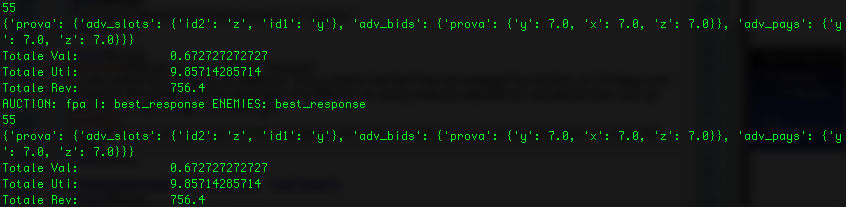
\includegraphics[scale=0.37]{img/revenuetheorem.png} 
\end{center}
\end{frame}

\subsubsection{Experiment on ``real case''}
\begin{frame}
\frametitle{Running Configuration}
\begin{itemize}
\item \textbf{Number of Query Words} 10
\item \textbf{Number of Auctions} 20
\item \textbf{Number of Slot for each word} [2, 4]
\item \textbf{Slot i click-through } [0,1]
\item \textbf{Number of Advertisers} 6
\begin{itemize}
\item 1 bot to test and 5 enemies (of the same kind)
\end{itemize}
\item \textbf{Values} [0, 20]
\item \textbf{Budgets}  [10, 50]
\item \textbf{Minimum Interest Threshold} [5, 15]
\item \textbf{Number of runs} 500
\end{itemize}
We choose two bots that have the best result among all the auction, and the worst one.
\end{frame}

\begin{frame}
\frametitle{Utility FPA}
\begin{center}
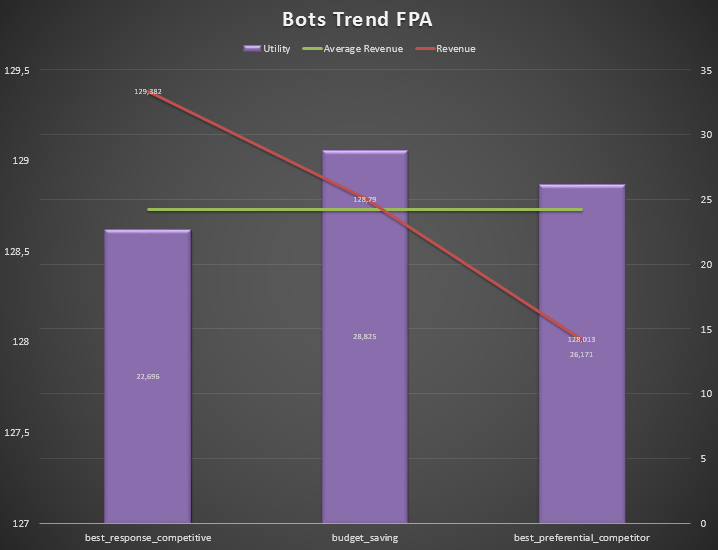
\includegraphics[scale=0.46]{img/Auctions/RFPA_all_Utility.PNG} 
\end{center}
\end{frame}

\begin{frame}
\frametitle{Heuristic FPA}
\begin{center}
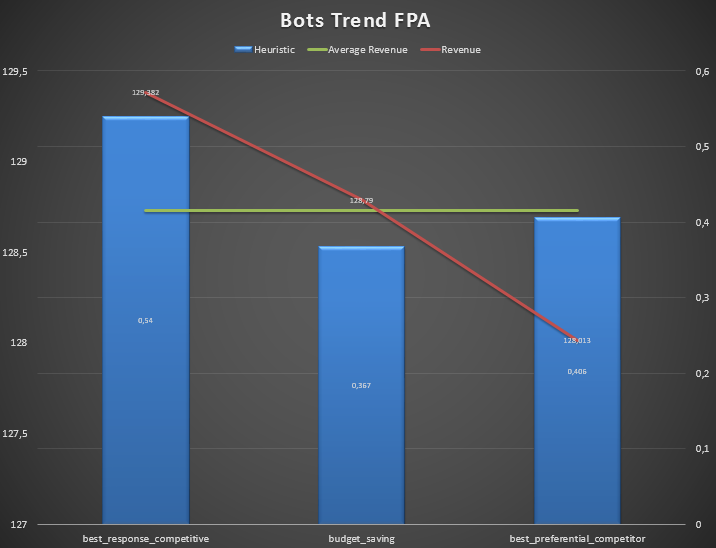
\includegraphics[scale=0.46]{img/Auctions/RFPA_all_Heuristic.PNG} 
\end{center}
\end{frame}

\begin{frame}
\frametitle{Consideration on FPA}
As expected the utility shows the \alert{same} behaviour as in the fixed auction and difference on the revenue are almost irrelevant.\\
\medskip
We notice a \alert{worsening} on the best\_preferential\_competitor due the fact that his behaviour is based on the threshold, that can change on different runs, this leading to more variability. 
\end{frame}

\begin{frame}
\frametitle{Utility GSP}
\begin{center}
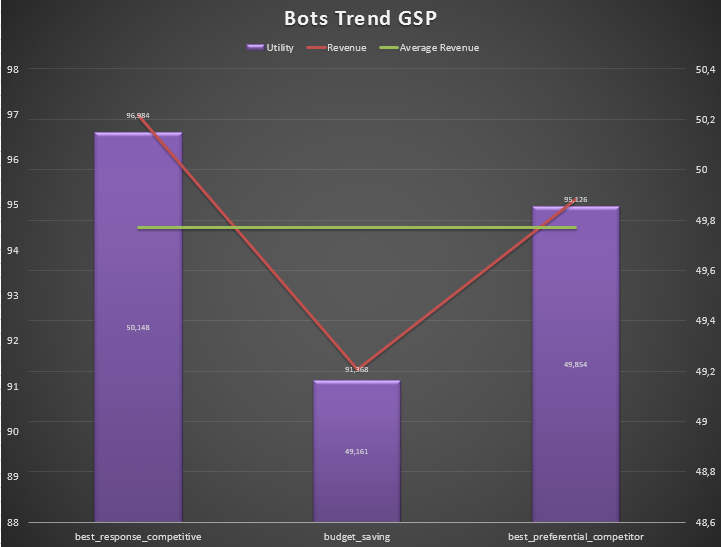
\includegraphics[scale=0.46]{img/Auctions/RGSP_all_Utility.PNG} 
\end{center}
\end{frame}

\begin{frame}
\frametitle{Heuristic GSP}
\begin{center}
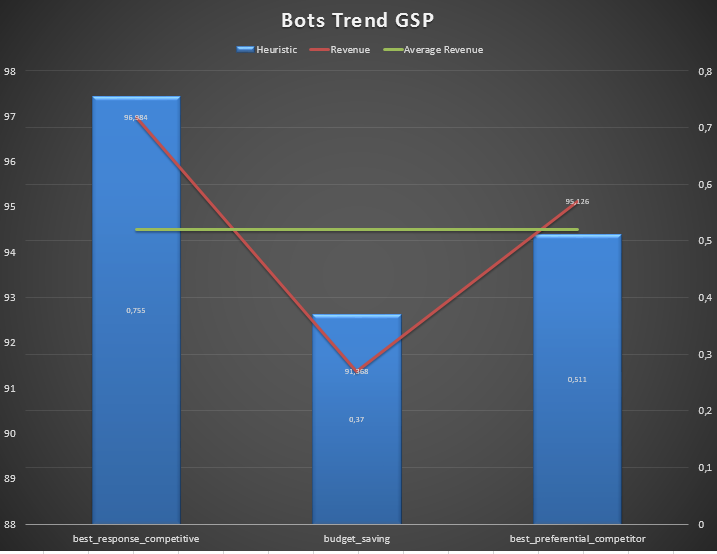
\includegraphics[scale=0.46]{img/Auctions/RGSP_all_Heuristic.PNG}
\end{center}
\end{frame}

\begin{frame}
\frametitle{Consideration on GSP}
In regards to utility and revenue, we notice that GPS shows the \alert{same} behaviour, as said in FPA best\_prefential\_competitor shows a \alert{worsening} for the same reason.\\
\medskip
Instead budget\_saving \alert{improves} his behaviour, still remaining the worst, because in each run the budget is not fixed.
\end{frame}

\begin{frame}
\frametitle{FPA vs GSP}
As seen in the fixed example, we can observe that:
\begin{itemize}
\item FPA lead to a \alert{higher} revenue compared to GPS
\item GPS hold a \alert{higher} utility and heuristic in relation to FPA
\end{itemize}
\end{frame}

\section{Summing UP}
\begin{frame}
\frametitle{Summing UP}
Based on all the experiments taken we can assume that the best configuration for a search engine  is:
\begin{itemize}
\item \textbf{Ranking}: indifferent since choice is based on what we are more interested in
\item \textbf{Matching}: Improved Best Match, since is quicker and gives the same result
\item \textbf{Auction}: 
\begin{itemize}
\item For the advertiser GSP
\item For the seller FPA
\end{itemize}
\end{itemize}
\end{frame}

\begin{frame}
\centering 
\Huge{Thank you for the attention.}
\end{frame}

\end{document}